\section{Fehler, Kosten und Qualitätsmaßnahmen}

% kurze Einleitung zum Thema
In diesem Kapitel wird auf die Fehler, Kosten und Qualitätsmaßnahmen eingegangen.
Hierzu werden typische Faults und Defects des Produkts beschrieben.
Diese werden durch Fehlerschwere, Priorität und potenzielle Fehlerkosten klassifiziert. 
Anschließend werden mehrere Methoden dargestellt, wie die Qualitätskosten in der Entwicklung gesenkt werden können.
Außerdem wird erörtert, warum es nicht sinnvoll ist eine vollständige Fehlersicherheit anzustreben.
Abschließend wird für das Produkt eine \ac{FMEA} durchgeführt.

\subsection{Faults und Defects}
% Beschreiben Sie typische Faults and Defects Ihres Software-Produkts. Stellen Sie Fehlerschwere, Priorität und potentielle Fehlerkosten dar.
% Notizen: 
    % Error: Fehlhandlung (Menschliche Handlung die zu einem nicht korrektem Resultat führt Beispiel: Programmierer – Fehler in Programmcode.)
    % Fault: Fehlerzustand (Auftreten eines Fehlers in der Software.)
    % Failure (/Defect): Fehlerwirkung (Bei der Programmausführung kommt es zu einem Abbruch  oder bestimmte Funktionen können nicht wie spezifiziert ausgeführt werden.)

% Aufgaben Aufbau:
    % Faults und Defects [] (-> Tabelle?)
        % Fehlerschwere (1-5) (Prio auch noch mit rein?)
        % Priorität
        % potentielle Fehlerkosten
Im folgenden Abschnitt werden die typischen Faults und Defects des DEV-CHAT's dargestellt.
Zusätzlich werden die Fehlerschwere, Priorität und potentielle Fehlerkosten identifizert und dargestellt.
Dies ist in der Tabelle \ref{tab:FaultsAndDeffects} dargestellt.
Die Fehlerschwere wird aus Nutzersicht beschrieben und teilt sich in fünf Kategorien die in der nachfolgenden Auflistung definiert werden.
\begin{enumerate}
    \item Systemabsturz mit ggf. Datenverlust
    \item Wesentliche Funktion fehlerhaft
    \item Funktionale Einschränkung / Abweichung
    \item Geringfügige Abweichung
    \item Schönheitsfehler
\end{enumerate}
Die Priorität beschreibt die Dringlichkeit der Behebung aus Projektsicht.
Diese wird in drei Kategorien aufgeteilt und ebenfalls in der nachfolgenden Auflistung definiert.
\begin{enumerate}
    \item Unmittelbar zu beheben
    \item Fehlerbehebung in nächster regulärer Version
    \item Fehlerbehebung erfolgt bei nächster Überarbeitung
\end{enumerate}
\begin{table}[H]
  \centering
    \begin{tabular}{l|c|c|c}
        \multirow{2}{*}{\textbf{Beschreibung}}                & \textbf{Fehler-} & \multirow{2}{*}{\textbf{Priorität}} & \textbf{Fehler-} \\
                                                              & \textbf{schwere} &                                     & \textbf{kosten}  \\ \hline
        Login nicht möglich                                   & 2             & 1         & mittel       \\ \hline
        Netzwerkverbindung bricht ab                          & 2             & 3         & hoch         \\ \hline
        Registrierung nicht möglich                           & 2             & 1         & mittel       \\ \hline
        Fehlerhafte Darstellung auf kleinen Displays          & 5             & 2         & gering       \\ \hline
        Beitreten eines Chatraums nicht möglich               & 3             & 1         & mittel       \\ \hline
        Benutzerrechte werden nicht korrekt interpretiert     & 3             & 1         & mittel       \\ \hline
        Passwortwechsel nicht möglich                         & 3             & 2         & gering       \\ \hline
        Chatnachricht kann nicht empfangen / versendet werden & 2             & 1         & hoch         \\ \hline
        Kurzbefehl wird nicht richtig ausgeführt              & 3             & 3         & gering       \\ \hline
        Webseite ist nicht erreichbar                         & 2             & 1         & hoch         \\ \hline
        Nachrichten-Latenz ist zu hoch                        & 4             & 2         & mittel       \\ \hline
        System ist überlastet                                 & 3             & 2         & hoch         \\ \hline
        System stürzt ab                                      & 1             & 3         & hoch        
    \end{tabular}
    \caption{typische Faults and Defects}
    \label{tab:FaultsAndDeffects}
\end{table}



\subsection{Qualitätskostensenkung und Fehlertoleranz}
Um Qualitätsbezogene Kosten zu reduzieren, muss zunächst die Zusammensetzung dieser dargestellt werden.
Qualitätskosten setzen sich aus den drei Bereichen Fehlerkosten, Fehlerverhütungskosten und Prüfkosten zusammen.
Fehlerkosten sind Kosten, die nach der Auslieferung des Produkts entstehen, wie z.B. Kosten für Reklamationen oder Vertragsstrafen.
Fehlerverhütungskosten sind Kosten die primär im Bereich des Qualitätsmanagements anfallen.
Prüfkosten entstehen in der Entwicklung bzw. Produktion, um das Produkt vor der Auslieferung zu Testen.
Die Fehlerverhütungskosten und Prüfkosten können zusammengefasst werden, da diese während der Entwicklung entstehen, die Fehlerkosten hingegen entstehen nach der Auslieferung des Produkts.
\newparagraph
Betrachtet man nun die Fehlerkosten in Relation zu den Fehlerverhütungs- und Prüfkosten lässt sich ein Zusammenhang erkennen.
Wird während der Entwicklung Wert auf eine hohe Qualität gelegt, entstehen höhere Qualitätskosten im Bereich Fehlerverhütungs- und Prüfkosten. 
Somit verringern sich die entstehenden Fehlerkosten, da durch die hohe Produktqualität mit weniger Beschwerden am ausgelieferten Produkt gerechnet werden kann.
Dieser Zusammenhang wird in Abbildung~\ref{fig:QKostenVerhaeltnis} dargestellt.
\begin{figure}[H]
    \centering
    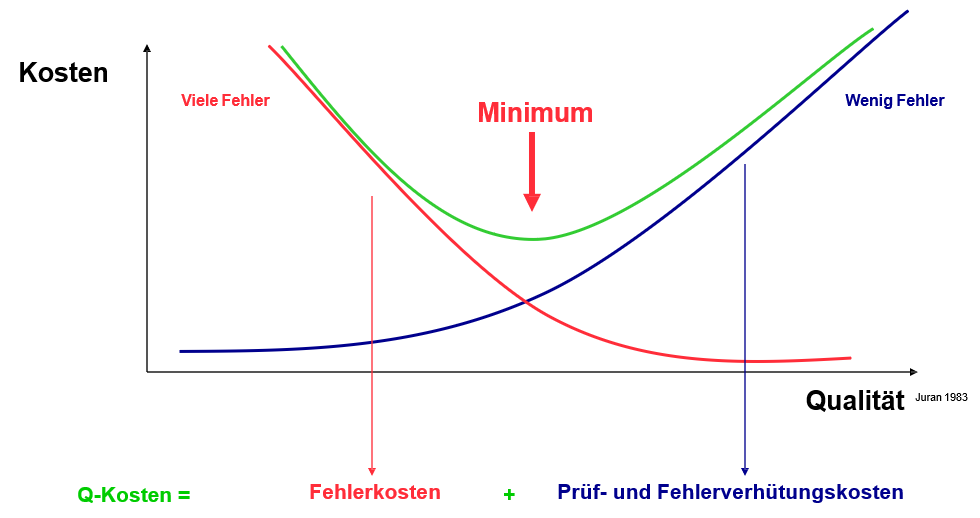
\includegraphics[width=1\textwidth]{images/qkostenverhaeltnis.png}
    \caption{Qualitätskosten Verhältnis}
    \label{fig:QKostenVerhaeltnis}
\end{figure}\noindent
% Wie Qualitätskosten in der Entwicklung senken?
% - S.28
% Warum nicht komplette Fehlerfreiheit?
Um die Qualitätskosten in Summe zu reduzieren, muss das perfekte Mittel zwischen den Fehlerverhütungs- und Prüfkosten und den Fehlerkosten gefunden werden.
Unter Berücksichtigung dieses Zusammenhangs wird ebenfalls klar, dass eine vollständige Fehlerfreiheit aus Kostensicht nicht sinnvoll ist.
Der Aufwand im Bereich der Fehlerverhütungskosten und Prüfkosten wächst exponentiell im Verhältnis zur Qualität während sich die Fehlerkosten nur langsam der Nulllinie annähern.
\newparagraph
Die Reduzierung der Qualitätskosten teilt sich in die zwei Bereiche Prozessverbesserung und Produktverbesserung.
Bei der Prozessverbesserung wird der Entwicklungsprozess optimiert.
Die Kostendynamik in einem Entwicklungsprozess wird in der auf Barry Boehm zurückgehenden Kostenkurve beschrieben.
Diese ist in Abbildung \ref{fig:boehm} dargestellt.
Die Kostendynamik bei einem Entwicklungsprozess verhält sich exponentiell.
Software wird in den klassischen Vorgehensmodellen innerhalb eines Projekts in den sechs Phasen Analyse, Entwurf, Implementierung, Test, Inbetriebnahme und Wartung entwickelt.
Das Ziel ist, dass bereits in der Analyse alle Anforderungen an die zu entwickelnde Software identifiziert werden.
Änderungen, die nach dem Entwurf der Software entstehen, können meist nur mit hohem Kostenaufwand berücksichtigt werden.
\autocite[vgl.][S. 95]{witte_testmanagement_2019}
\begin{figure}[H]
    \centering
    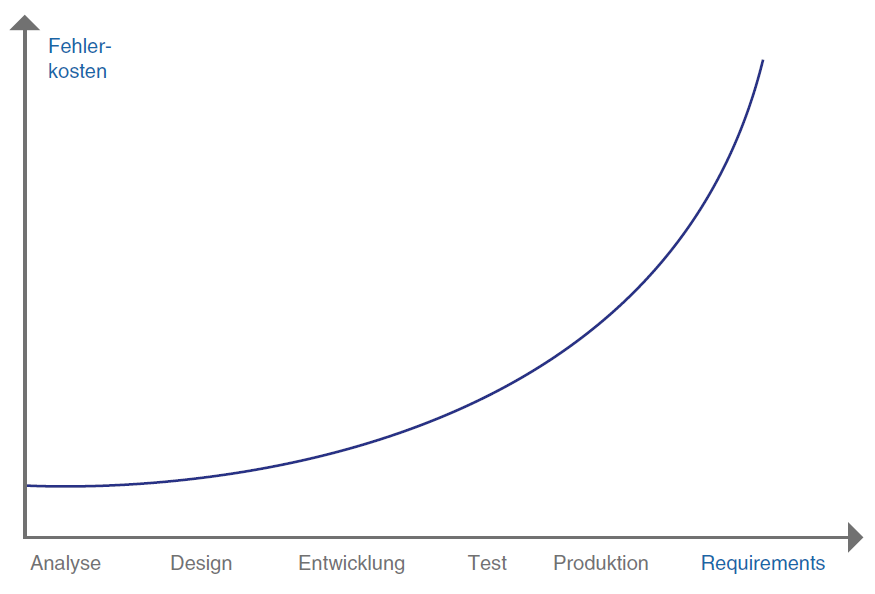
\includegraphics[width=0.8\textwidth]{images/boehm.png}
    \customcaption{Kostenkurve Barry Boehm}{\autocite[][S. 97]{witte_testmanagement_2019}}
    \label{fig:boehm}
\end{figure}\noindent
Die Verbesserung des Entwicklungsprozesses erfolgt im Rahmen eines \ac{KVP}.
Hierbei kann die PDCA-Methode verwendet werden.
Diese setzt sich aus den Phasen \textbf{P}lan, \textbf{D}o, \textbf{A}ct und \textbf{C}heck zusammen, welche nachfolgend beschrieben werden.
\begin{quote}
    \textbf{Plan}: Analyse der aktuellen Situation und gewünschten Situation, Identifikation der Verbesserungspotentiale, Maßnahmen entwickeln zur Erreichung des Zielzustands.\\
    \textbf{Do}: Durchführug der geplanten Maßnahmen.\\
    \textbf{Check}: Vergleich Sollzustand und Istzustand.\\
    \textbf{Act}: Abhängig davon, ob die Maßnahmen erfolgreich sind, werden diese als Standard definiert oder der Prozess wird erneut durchlaufen.
\end{quote}
Da DEV-CHAT einmalig in der Vorlesung Software-Engineering entwickelt wurde, wird es einen weiteren Entwicklungsprozess mit dieser Teamkonstellation nicht geben, weshalb eine Prozessoptimierung nur theoretisch durchgeführt werden kann.
Die Probleme und die zugeordneten Maßnahmen der Plan Phase werden in Tabelle~\ref{tab:pdca} dargestellt.
\begin{table}[H]
  \centering
  \begin{tabular}{l|l|l}
    \textbf{Problem} & 
    \textbf{Beispiel} & 
    \textbf{Maßnahme} 
    \\\hline
    \multirow{3}{.25\textwidth}{nicht korrekte Verwendung von Scrum} & 
    \multirow{3}{.35\textwidth}{Scrum Master und Product Owner gleichzeitig Developer} & 
    \multirow{3}{.3\textwidth}{Schulung zu Scrum} 
    \\
    &&\\
    &&\\\hline
    \multirow{4}{.25\textwidth}{Architektur unklar bei Implementierung} &
    \multirow{4}{.35\textwidth}{Änderungen an der grund\-le\-gen\-den Softwarearchitektur während der Implementierung} & 
    \multirow{4}{.3\textwidth}{vollständige Entwicklung der Architektur vor Begin der Implementierung} 
    \\
    &&\\
    &&\\
    &&\\\hline
    \multirow{3}{.25\textwidth}{mangelndes Wissen über verwendete Technologien} & 
    \multirow{3}{.35\textwidth}{erstes Projekt mit React.js und Next.js, deshalb nicht voller Umfang ausgenutzt} & 
    \multirow{3}{.3\textwidth}{Einführung in Technologien, ggf. externe Schulung}
    \\
    &&\\
    &&\\\hline
    \multirow{3}{.25\textwidth}{mangelhafte Verwendung von Bibliotheken} &
    \multirow{3}{.35\textwidth}{eigenständige Programmierung von Authentifizierung, FrontEnd Komponenten} & 
    \multirow{3}{.3\textwidth}{umfassende Analyse von Bibliotheken zu Funktionen (Npm-Paketmanager)}
    \\
    &&\\
    &&\\ 
  \end{tabular}
  \caption{Übersicht Probleme und Maßnahmen}
  \label{tab:pdca}
\end{table}\noindent
In weiteren Schritten müssten diese Maßnahmen nun durchgeführt und evaluiert werden.
Alternativ zu der PDCA-Analyse kann auch \ac{CMMI} verwendet werden, auf welches in dieser Arbeit nicht tiefer eingegangen wird.
\newparagraph
Bei der Produktverbesserung wird die Qualität des tatsächlichen Produkts verbessert.
Da DEV-CHAT nur im Rahmen der Vorlesung entwickelt wurde und nicht veröffentlicht wird, ist eine Qualitätsoptimierung auch nur theoretisch durchführbar. 
Sollte eine Weiterentwicklung bzw. eine Veröffentlichung erfolgen, sollten die Untenstehenden Punkte abgearbeitet werden.
\begin{itemize}
    \item Erweiterung der UnitTests, bisher nur Exemplarisch
    \item Blackbox Test zur Usability
    \item Database Monitoring
    \item Vollständige Umsetzung von Websockets, mit Fallback (zyklische Abfragen)
\end{itemize}

\subsection{\acl{FMEA}}
\label{sec:FMEA}
% Failure Mode and Effects Analysis (FMEA) (realistische Annahme für Risikoprioritätszahl RPZ
Im folgenden wird für den DEV-CHAT eine \ac{FMEA} durchgeführt.
\gqq{
    Ziel der FMEA ist es, bei der Entwicklung eines Produktes bzw. der Bearbeitung einer Aufgabe mögliche Fehler frühzeitig zu erkennen, um die Funktion sowie die Sicherheit und eine hohe Produkt- bzw. Prozessqualität gewährleisten zu können.
    Durch die frühzeitige Erkennung können sowohl die Anlaufkosten und die entstehenden Kosten infolge von Rückrufaktionen und Reklamationen reduziert werden als auch die Entwicklungszeit verkürzt werden
} \autocite[][]{noauthor_fmea_nodate}.
\newparagraph
Die \ac{FMEA} lässt sich grob in zwei Schritte aufteilen, in die Ermittlung der Funktionen des Produkts und die anschließende Analyse dieser Funktionen.
Ausgehend von der Analyse können somit Schwachstellen aufgedeckt werden und mögliche Lösungsvorschläge erarbeitet werden.
Die Ermittlung der Funktionen kann in einem Strukturdiagramm dargestellt werden.
Dies wurde bereits in Abbildung~\ref{fig:Produktstruktur} dargestellt.
Die Analyse erfolgt in einer Tabelle, welche in Abbildung~\ref{fig:FMEA} dargestellt ist.
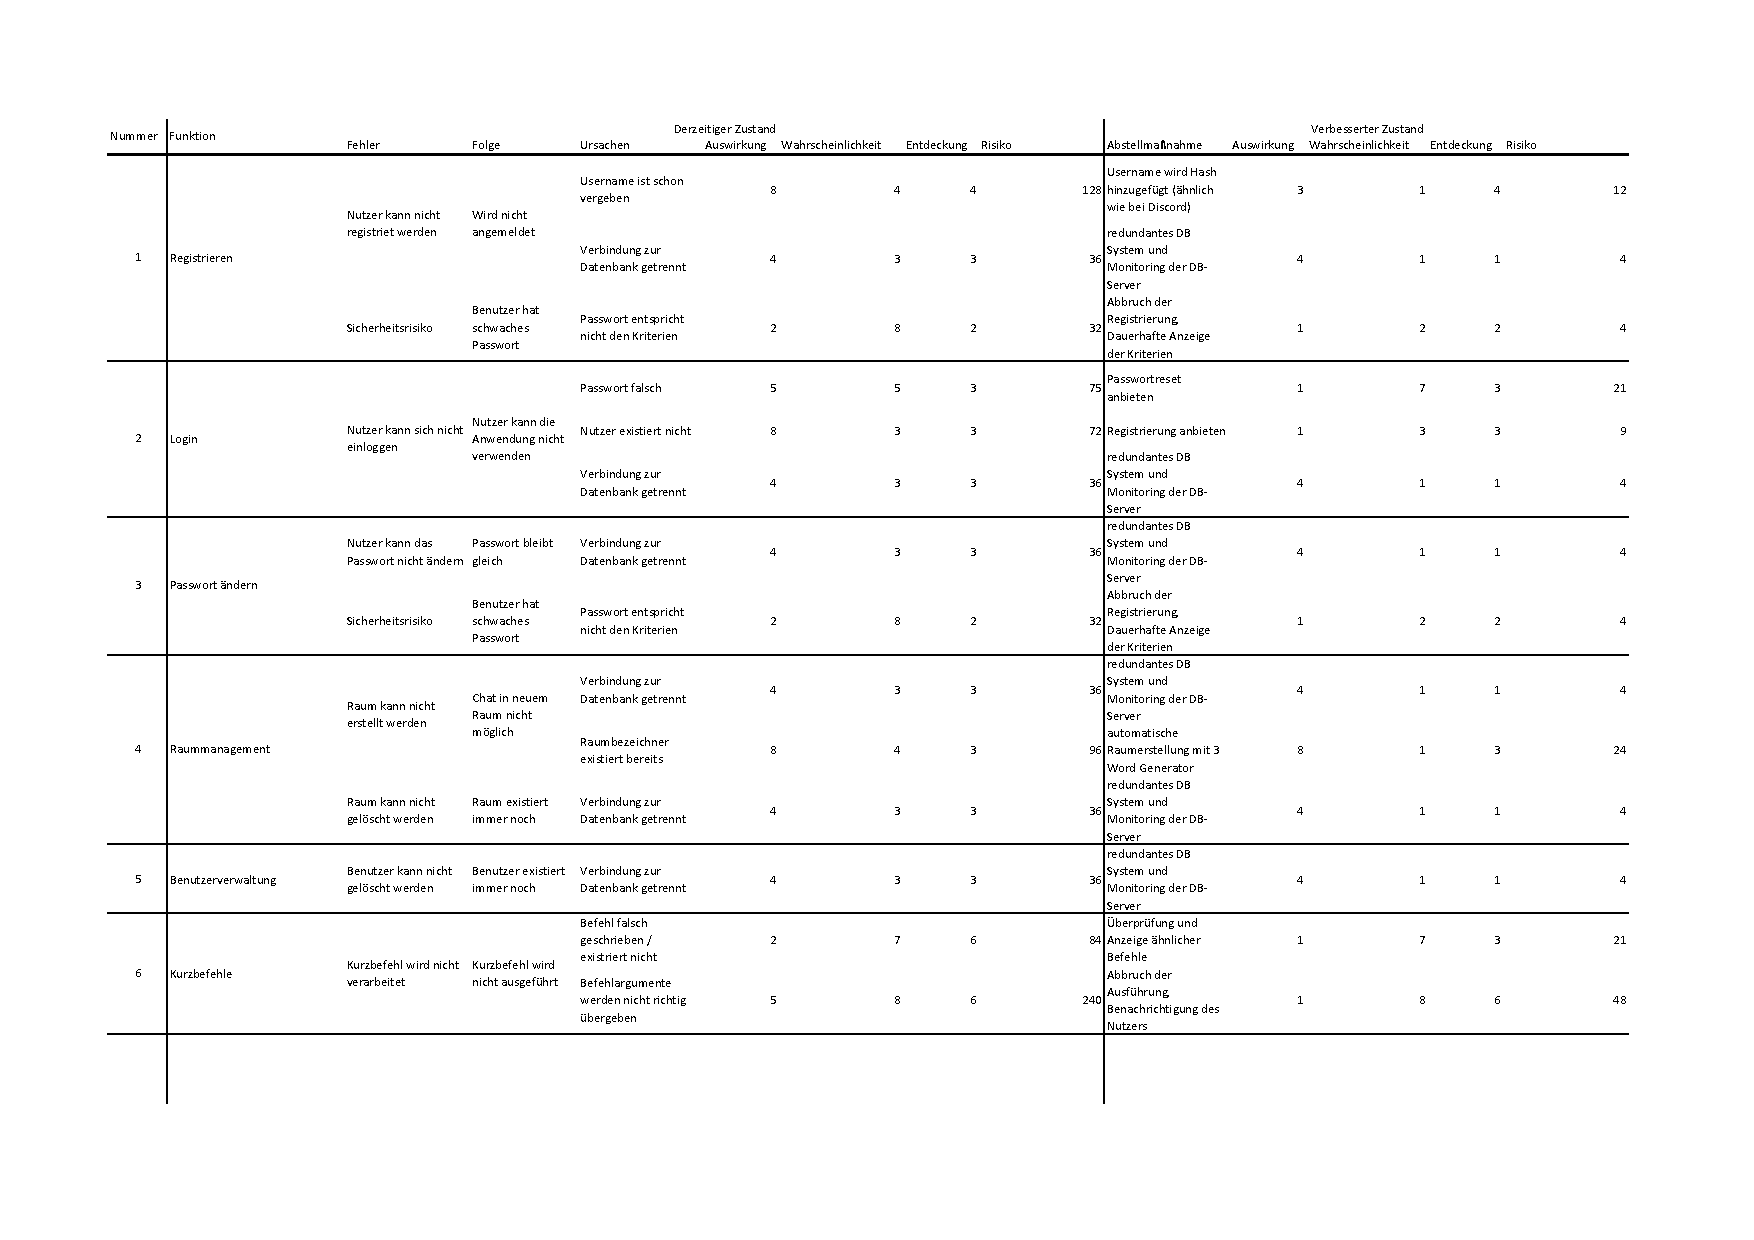
\includepdf[pages=1, pagecommand=\label{fig:FMEA}, scale=0.8, angle=90, offset=0 0]{images/fmea_export.pdf}
\includepdf[pages=2, scale=0.8, angle=90, offset=0 0]{images/fmea_export.pdf}



